In this chapter, the review of literature relevant to the study area of the heart disease prediction using machine learning techniques is carried out and one of the major focuses is to explain the history and empirical basis of this study.

\section{Heart disease}
Heart disease is a term used to represent a variety of illnesses or conditions that affect the heart, including coronary artery disease, heart rhythm issues (arrhythmias), hereditary defects (congenital heart defects), heart valve disease, diseases of the heart muscle, and infections of the heart. Heart disease can be caused by things like underlying health problems, contamination, irritation, and family history. To help prevent cardiovascular disease, you should live a healthy lifestyle and stay away from smoking, food that makes you fat, and stress. Heart disease is a serious problem in many countries around the world.

\subsection{Typical heart problems}

The factors that cause the heart to break down include any major abnormal heart or blood vessel condition known as coronary disease. The different sorts of heart disease are:

\begin{enumerate}[label=(\alph*)]
	\item{Coronary Artery Disease: refers to arrangement of cholesterol plaque which causes solidifying or restricting of the heart channel, (which supplies blood to the heart).}
	\item{Cardiomyopathy: refers to a disease of the heart muscle that makes it harder for the heart to pump blood to the rest of the body.}
	\item{Angina: a type of chest pain caused by reduced blood flow to the heart.}
	\item{Valvular Heart Disease: refers to damage or decease on at least one of the four valves of the heart.}
	\item{Congenital Heart Disease: refers to a variety of birth defects that affect the normal functioning of the heart.}
	\item{Heart attack: A heart attack occurs when an artery carrying blood and oxygen to the heart becomes blocked.}
	\item {Heart failure: Heart failure occurs when the heart muscle fails to adequately pump blood. This does not mean the heart has stopped beating. }
	\item{Arrhythmia: An alteration in the heart's electrical impulse sequence that can cause irregular or fast (tachycardia) or slow (bradycardia) heartbeats. }
	\item{Rheumatic Heart Disease: a condition where the heart muscles and valves are permanently damaged due to rheumatic fever.}
	
	\item{Ischemic Heart Disease (IHD): is the term given to heart problems caused by narrowed heart arteries.}
	
\end{enumerate}

\subsection{Symptoms of heart disease}
The above-mentioned heart diseases are only a few of the many heart diseases that affect both men and women. These can be detected by paying close attention to the common factors that cause heart disease. The following are some of the most prevalent symptoms of heart disease:

\begin{enumerate}[label=(\alph*)]
	\item{Having pain in the upper body such as the arms, jaw, neck, back or upper stomach.}
	\item{Significant strain, discomfort, or a burning pain in the chest.}
	\item{Rapidly expanding heartbeat.}
	\item{Unsteadiness, sweating and nausea.}
	\item{Swelling, anxiety, cough, aching, burning and so on...}
\end{enumerate}

\subsection{Cure of heart disease}
According to \citefullauthor{Clinic2022Can}, unfortunately, there is no cure for coronary heart disease, and once recognized, the illness cannot be reversed. However, one can make lifestyle adjustments to minimize their chances of having other health issues, such as a heart attack.

\section{Machine Learning}
Machine learning is a branch of artificial intelligence that is focused on making systems that can learn from their experiences and make predictions based on what they have learned. It uses a training dataset to teach machine learning algorithms so that a model can be made. With the new information, the model can predict heart disease. Using machine learning, it looks for hidden patterns in the input dataset to build models. It can accurately predict what will happen with new data sets. The data set is cleaned up, and values that are missing are added. The model uses the new data to make predictions about heart disease, which are then tested to see how well they work. 

\subsection{Techniques for machine learning}
Techniques for machine learning can be grouped into supervised learning, unsupervised learning, and reinforcement learning.

\subsubsection{Supervised learning}
The model is trained on a labelled data set. The dataset contains the inputs and an outcome. Data are sorted and separated into training datasets and test datasets. Training dataset is used to train our model, and testing dataset is used as new data to test how well the model works. 
A good example of this is the classification and regression.
\subsubsection{Unsupervised learning}
The data set does not contain any classed or labelled data used for training. The objective is to uncover patterns within the data. The model has been taught to create patterns. It can quickly identify hidden patterns in every new input dataset, but after further data exploration, it uses the datasets to derive conclusions about hidden patterns.
With this method, the dataset has no responses. An example of an unsupervised learning method is the clustering approach.
\subsubsection{Reinforcement learning}
In this method, the model refines its presentation based on its association with the environment. It doesn't use labelled datasets, and neither the results nor the data are linked to the datasets. Instead, the model learns from what it does. It also determines how to disclose its flaws and how to attain the desired conclusion by assessing and testing a variety of potential outcomes.
Classification algorithms are a popular type of supervised learning technique that are used to determine the likelihood of an individual having heart disease.


\subsection{Classification Machine Learning Techniques}
To classify something means to recognize it, comprehend it and place it in a set of categories that have already been established. Machine learning programs utilize several algorithms. Machine learning systems use multiple methods to classify new datasets based on previously classified training datasets. The following subsections discuss the algorithms used in this study.

\subsubsection{Logistic regression}
Classification algorithms, such as logistic regression, are supervised.
This statistical model is frequently employed in categorization and predictive analytics. Based on a collection of independent variables, logistic regression calculates the likelihood that a certain event will occur. 

As a result, the dependent variable is limited to a range of 0 to 1. 
Independent variables are analysed to determine the binary outcome with the results falling into one of two categories. The independent variables can be categorical or numeric, but the dependent variable is always categorical. Written like this: $$P(Y=1|X) or P(Y=0|X)$$
It calculates the probability of dependent variable Y, given independent variable X. 


\subsubsection{Naive Bayes}
Naïve Bayes  is a machine learning algorithm used to solve classification problems. Naïve Bayes is based on the Bayes Theorem and is one of the simplest yet powerful ML algorithms in use. It finds applications in many industries.

The Bayes' theorem is used by Naïve Bayes algorithm, which also assumes that each predictor is independent. To put it another way, this classifier makes the assumption that the presence of one specific feature in a class has no influence on the presence of another.

\begin{figure}[htb]
	\centering
	\makebox[0cm]{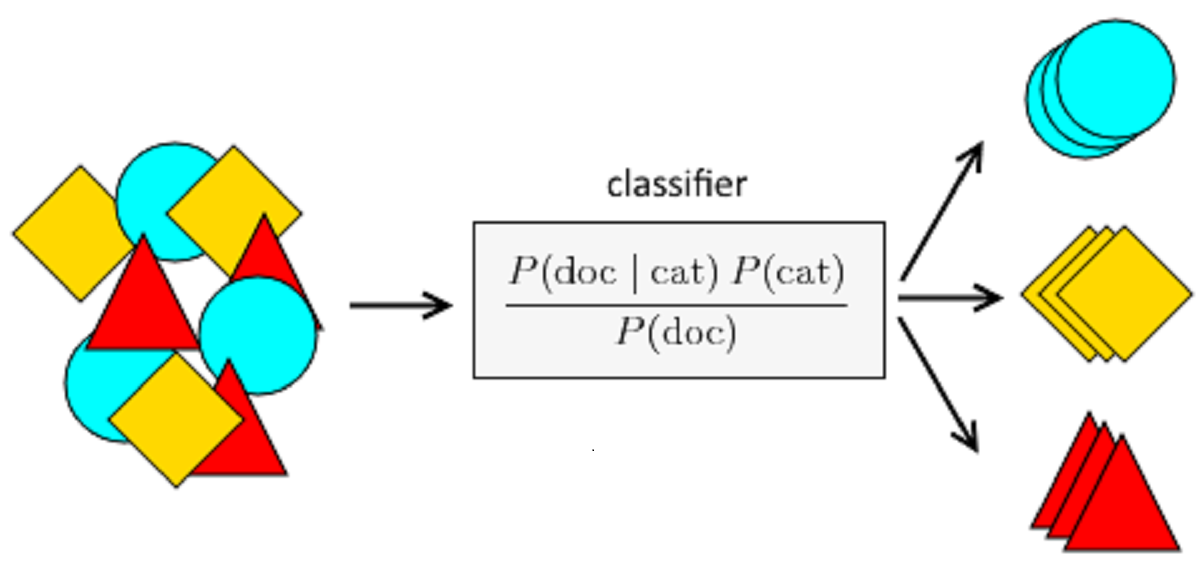
\includegraphics[scale=0.5]{nb.png}}
	\caption{Naive bayes}
	\label{fig:nb}
\end{figure}

\subsubsection{K-nearest neighbours}
The K-nearest neighbors (KNN) algorithm is a form of supervised learning technique that can be used for regression as well as classification. KNN performs a distance calculation between the test data and all of the training points in an effort to determine which class the data being evaluated should be assigned to. The K number of points that should be selected is the one that comes closest to the test data. The KNN algorithm computes the chance that the test data belong to the same classes as the 'K' training data, and the class that retains the highest probability is the one that is chosen. In the case of regression, the value is determined by calculating the average of the 'K' training points that were chosen.

Say we have a picture of something that looks like both a cat and a dog, but we want to know if it's a cat or a dog. We can use the KNN method for this identification because it measures similarity. Our KNN model will look for similarities between the new data set and the images of cats and dogs. Based on the similarities it finds, it will put the new data set into either the cat or dog category.

\begin{figure}[htb]
	\centering
	\makebox[0cm]{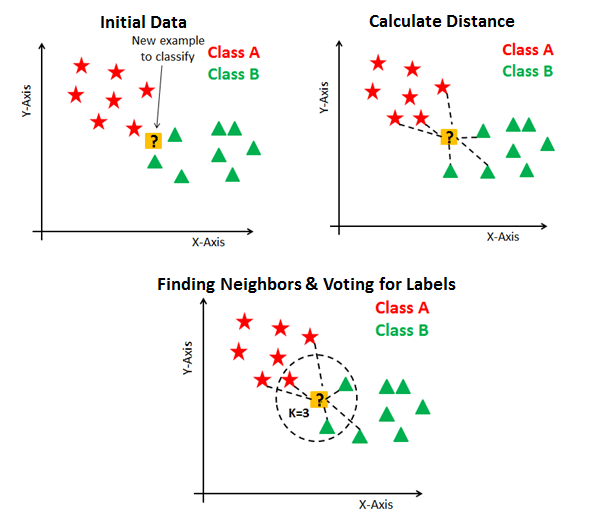
\includegraphics[scale=0.45]{KNN.png}}
	\caption{K-nearest neighbours}
	\label{fig:knn}
\end{figure}

\subsubsection{Decision Tree}
A decision tree is a non-parametric supervised learning algorithm that can be used for both classification and regression tasks. As a supervised learning technique, a decision tree is ideal for classifying issues at a precise level of detail. Like a flow chart, it takes data from the "tree trunk" and divides it into two related categories at a time: "branches" and "leaves." This allows for organic classification with minimal human oversight by creating categories within categories.

\comment{
	\begin{figure}[htb]
		\centering
		\makebox[0cm]{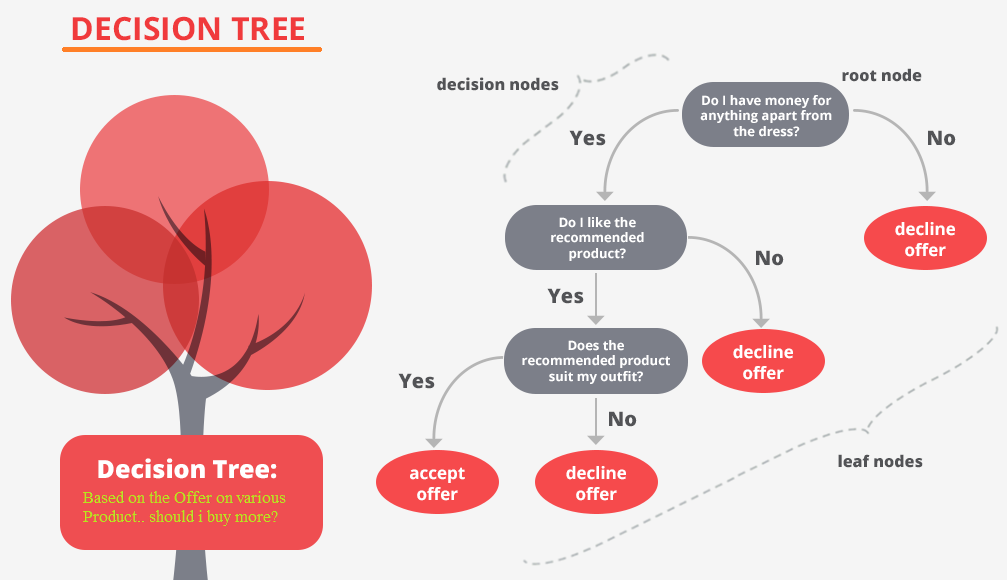
\includegraphics[scale=0.45]{dt.png}}
		\caption{Decision tree}
		\label{fig:dt}
	\end{figure}
}


\comment{

\section{Machine learning}
Machine learning is a subfield of artificial intelligence (AI) and computer science that uses data and algorithms to mimic how humans learn, gradually improving its accuracy. It primarily focuses on teaching computers to learn and adapt from real facts and data while also improving with experience.

\subsection{Benefits of machine learning in medicine}
Here are some benefits of machine learning in medicine.
\begin{enumerate}
	\item{Improves in disease identification and diagnosis.}
	
	\item{Helps in drug discovery and manufacture.}
	
	\item{Improved radiotherapy.}
	
	\item{Predictions of outbreaks.}
	
	\item {Prediction of liver and cardiovascular disease.}
\end{enumerate}d
}
\section{Related works}{
\setlength{\parskip}{1em}

\citealp{taneja2013heart}, applied data mining and AI calculations to be specific, Decision Tree (J48 calculation), Artificial Neural Networks (ANN), Naive Bayes, and for heart illness forecast. A dataset of 7339 occasions with 15 elements has been selected from PGI Chandigarh. WEKA 3.6.4 instrument was utilized for the test. For model preparation and testing 10-Fold, Cross-Validation strategies are utilized arbitrarily. Best First Search strategy was utilized to select the most ideal attributes from the available 15 ascribes and among them just 8 attributes have been chosen. Each experiment was finished in two distinct situations, the initial one containing each of the 15 attributes and the second case just 8 selected attributes.

\citealp{yan2006multilayer} fostered a multiplayer perceptron-based choice help system to help the determination of coronary heart disease. The input layer of the system includes 40 input variables, categorized into four groups and then encoded using the proposed coding schemes. The number of nodes in the hidden layer is determined through a cascade learning process. In the system, the missing data of a patient are handled using the substituting mean method. A total of 352 medical records collected from the patients suffering from five heart diseases have been used to train and test the system. The results show that the proposed MLP-based decision support system can achieve very high diagnosis accuracy greater than (90\%) and comparably small intervals less than (5\%), proving its usefulness in support of clinic decision process of heart diseases.

\citealp{setthukkarase2012intelligent} fostered another neutral fluffy strategy to analyze current realities of the illness in patients reports. The summed-up database is designed for decision-production from a diminished arrangement of qualities, which is the result of the hereditary calculation. Four layered fluffy neutral networks are utilized for effective displaying and surmising with time reliance under vulnerability.

\citealp{dangare2012improved} carried out a system for foreseeing heart disease and has applied three data mining order procedures: Decision trees, Naive Bayes and Neural Networks. The outcomes show that neutral networks are better than decision trees and Naive Bayes.

\citealp{waghulde2014genetic} performed heart disease informational collection regarding multi-facet neutral networks related to back spread learning calculations for network preparing. A weighting calculation is utilized to improve neutral network initialization. This study shows the consequences of the Genetic Neural Network for heart illness expectation, utilizing an ideal neutral network design that predicts whether a patient is experiencing coronary illness, further developing accuracy by 98%

\citealp{sudha2012effective} concentrated on arrangement calculations, for example, Decision tree and Naive Bayes to distinguish stroke disease. Classification methods, for example, decision trees, Bayesian classifiers, and backpropagation neutral networks were utilized in this review. Records with irrelevant information were erased from the information distribution center before the mining system occurred.

\citealp{ordonez2001mining} studied on the prediction of heart disease with the assistance of affiliation rules. They utilized a straightforward planning calculation. This algorithm regards attributes as numeric. It is utilized to change over clinical records into exchange designs. Improved calculations are utilized to minify confined affiliation rules. The mapping table is ready and the characteristic worth is planned to the item. Decision trees are utilized for data mining since they naturally partition numeric qualities. Split points chosen in the choice tree are seldom utilized. Grouping is utilized to acquire a general comprehension of the data


\citealp{babu2017heart}  have proposed that medical data mining can uncover hidden patterns in medical datasets. Clinical diagnosis could make good use of these patterns. Standardize data collection. Age, sex, blood pressure, blood sugar, and other medical profile factors can help in predicting heart disease risk. These features are input into K-means, MAFIA, and Decision tree classification in heart disease prediction, employing data mining to heart disease treatment; it can deliver a reliable performance in diagnosing heart disease. By doing so, medical industries can provide better patient diagnosis and treatment, improving service quality. This paper's key benefits include early detection, accurate diagnosis, and affordable treatment.


\citealp{pattekari2012prediction} designed an Intelligent System using the Naive Bayes modeling method for data mining. It is set up as a web-based application in which the user answers questions that have already been set up. It gets hidden data from the database where it is stored and compares the user's values with the trained data set. It can answer complicated questions about heart disease and help doctors make smart clinical decisions, which is something that traditional decision support systems can't do. It also helps to lower treatment costs by making sure that treatments work.

\comment{
Huiyan Wang (2008) has sought after a specialty in this sward by proposing a mechanized symptomatic model to advance normalization and promotion of conventional Chinese medication (TCM) finding. The system fills in as follows. First, the incidental effects are picked by acquiring the Bayesian association structure from a data set of cases that coordinate normal information speculation. In the design, the Markov blanket of the objective variable is chosen as the side effect set. Second, the planning connections between side effect sets and indicative results relies on naive Bayesian classifiers.

The next venture in the field was by Huang Jianyong (2004). This review aims to tackle the issue of multiclass grouping utilizing parallel classifiers. The paired characterization tree configuration is done so that the class group is separated into two distinct subsections from one hub. The hub takes on the class module strategy to further develop the binary characterization capacity. Partitioning is planned as an improvement issue, and, hereditary calculations are proposed to tackle advancement issues. Heart mumbles were a significant issue in pediatric cardiovascular illness, and this gathering  had a high occurrence of cardiovascular commotion (77\% - 95\% as reported), bringing about little blockage because of intrinsic coronary illness.
} 

\citealp{ismaeel2015using} attempts to replace the expensive clinical check-up by an advance warning system for patients that are probably going to experience the ill effects of heart disease. The proposed approach utilizes outrageous machine learning algorithm to show the different qualities of the dataset which is ongoing information gathered by the sever land clinical establishment containing 300 examples. The two machine learning technique Utmost Machine Learning and ANN were utilized for the investigation among which utmost Machine Learning shows the most highest precision of 87\%. The Utmost machine learning algorithm has five (0-4) results and utilizing this model, the analysis of new patient should be possible utilizing the past information.


%%%%%%%%%%%%%%%%%%%%%%%%%%%%%%%%%
%%%%%%%%%%%%%%%%%%%%%%%%%%%%%%%%
\comment{
Monika Gandhi et al (2015). The fundamental aim in this study is the mechanization of such system for diagnosing heart disease by thinking about earlier data and information. It plans to give details of different strategies of information deliberation by utilizing data mining techniques, including their benefits and negative marks.
}

\citealp{jabbar2013heart} proposed an approach which consolidates KNN with a Genetic model. The wellspring of the dataset is UCI AI repository including 5 attributes and 14 examples. The proposed model was not effective for essential growth and breast cancer because of immaterial and excess elements present in the dataset. The outcomes uncover the get-over rate for hereditary calculation is 60\% KNN, the review shows expansion in precision for expectation of coronary illness.


\citealp{deepika2011association} concentrated on Pruning-Classification Association Rule (PCAR) to remove affiliation rules. PCAR has given an analysis of the Apriori algorithm. PCAR covers a bunch of least frequency, which eliminate unpredictable things from a bunch of things. It then, at that point, sorts the arrangement of things in light of the recurrence of the arrangement of things and tracks down a successive arrangement of items. Ordonez utilizes affiliation rules in data mining to get better coronary illness prediction results. The authors concentrated on the limitation of affiliation rules that mined the whole data collection without check of autonomous samples. We presented calculations that changed the inquiry limitations to decrease the quantity of affiliations runs and approved them utilizing train and test approaches. They have concentrated on two corresponding tasks which are anticipating the absence and foreseeing the presence of coronary illness.

\citealp{srinivas2010applications} proposed the use of data mining strategies to the prediction of cardiovascular failure. The authors concentrated on grouping-based data mining strategies, for example, decision trees, rule-based, Naive Bayes, and artificial neural networks for a tremendous measure of clinical information. The Tanagra data mining apparatus was utilized to look at data investigation, machine learning, and measurable learning algorithms. They utilized a preparation informational collection of 3000 cases with 14 distinct properties. Examples of the informational collection address the results of different test types to anticipate the precision of coronary illness.

\citealp{sowmiya2021hybrid} acknowledge that it is crucial to have a system that can practically perceive the pervasiveness of coronary illness in countless tests immediately. The authors evaluated the ability of nine grouping strategies for the prediction of coronary illness. Specifically, decision tree, naive Bayesian neural network, SVM.ANN, KNN. The proposed algorithm of Apriori estimation and SVM (support vector machine) in coronary illness prediction. Utilizing clinical profiles, for example, blood pressure, fasting blood sugar, and chest pain type. It can foresee the likelihood of patients getting a coronary illness. Because of this, medical society checks out distinguishing and preventing coronary illness. The investigation it has exhibited that classification-based procedures contribute to high viability and acquire high exactness accuracy compared to the previous methods.

\citealp{sultana2016analysis}, created heart disease prediction utilizing KStar, SMO, j48, Bayes Net and Multilayer perception utilizing WEKA system. In light of execution from various component SMO and Bayes Net accomplish ideal execution than KStar, Multilayer perception and J48 strategies utilizing kfold cross approval. The exactness of these algorithms is additionally not agreeable. The precision of the outcomes is therefore improved to empower a superior indicative decision.

\citealp{raihan2016smartphone} has fostered a straightforward way of forecasting the probability of IHD utilizing a smartphone. The use of clinical data gathered from patients conceded with IHD has developed Android-based model applications. Clinical data from 787 patients was examined with risk factors, for example, hypertension, diabetes, raised cholesterol, smoking, obesity, depression, and current clinical side effects that might show the hidden unrecognized  IHDs. Data were separated and a score was produced utilizing data mining innovation Risks for IHD are reviewed as low, medium, and strong. The authors observed that a significant relationship among low-and medium-and high-grade cardiovascular occasions was noticed for patients whose data were gathered to deliver the evaluations, individually; p=0.0001 and 0.0001. They gave a basic approach to recognizing the risk of IHD and are inclined to cardiology to keep away from sudden deaths. As of now, there are a couple of constraints on the open resources that make them unused by the population.

\comment{
\citealp{babu2017heart} have proposed that medical data mining can uncover hidden patterns in medical datasets. Clinical diagnosis could make good use of these patterns. Standardize data collection. Age, sex, blood pressure, blood sugar, and other medical profile factors can help in predicting heart disease risk. These features are input into K-means, MAFIA, and Decision tree classification in heart disease prediction, employing data mining to heart disease treatment; it can deliver a reliable performance in diagnosing heart disease. By doing so, medical industries can provide better patient diagnosis and treatment, improving service quality. This paper's key benefits include early detection, accurate diagnosis, and affordable treatment.

}
According to \citealp{mohan2019effective}, Machine learning has been indicated to be viable in serving with simple choices and forecasts from the tremendous measures of data delivered by the medical services industry. Machine learning methods are being used in ongoing improvements in various regions of the Internet of Things (IoT). Different investigations give just a brief look into predicting heart disease with machine learning procedures. Authors proposed a clever methodology that targets tracking down huge elements by applying machine learning procedures bringing about working on the precision in the estimate of cardiovascular sickness. The prediction model is given different mixes blends of features and a couple of known grouping procedures. We produce an improved performance level with an accuracy level of 88.7\% through the prediction model for coronary illness with the hybrid irregular forest with a linear model (HRFLM).

\citealp{jabbar2016heart} said that heart disease is an overall driving reason for death. According to the authors, there is a need for an intelligent decision support system for for the prediction of heart disease is required. Strategies for data mining are additionally used to evaluate the patient's typical heart condition. Hidden Naive Bayes is a kind of data mining that reduces the conditional assumption of the usual Naïve Bayes. The model proposed noticed that the Hidden Naïve Bayes can be applied to the classification of heart disease. experimental results on heart disease data set show that the HNB records 100\% in terms of accuracy and out performs Naïve bayes.

According to \citealp{ed2019real}, early identification of heart disease and constant checking can decrease the mortality rate. The remarkable development of data from different sources, for example, wearable sensor gadgets utilized in Internet of Things health monitoring, streaming system, and others have been producing a colossal measure of data consistently. The combination of streaming huge data storage and machine learning is a cutting-edge innovation that can have a critical effect in the medical care field particularly early detection of coronary illness. This alteration can be even more astounding and more reasonable. A continuous heart disease prediction system has been proposed in light of Apache Spark. The system comprises two principal sub-parts, to be specific streaming processing and visualization.

\citealp{haq2018hybrid} have concocted a Hybrid Intelligent System for the Prediction of Heart Diseases. The authors declared that noninvasive-based techniques, for example, machine learning are dependable and proficient. A Machine-learning-based diagnosis system for heart disease prediction by utilizing a heart disease prediction dataset was created utilizing seven famous machine learning algorithms, three feature selection algorithms, the cross-approval technique, and seven classifiers execution assessment measurements like grouping exactness, explicitness, responsiveness, Matthews' relationship coefficient, and execution time. The proposed system can undoubtedly distinguish and arrange individuals with heart disease from healthy people. Furthermore, receiver optimistic curves and regions under the bends for every classifier were figured. The authors validated the performance of the proposed system on full elements and a diminished arrangement of elements. The component decrease affects classifier execution to the extent that precision and execution time of classifiers.

\citealp{satu2018exploring}, present that heart disease is one of the main infections that cause huge loss of lives from one side of the country to the other. A couple of astonishing ways of figuring out basic factors of heart contaminations have been seen by the creators. Values of the different extent of individual attributes in these data are determined to figure out significant components of this affliction. Then, semi-regulated learning algorithms, for example, Collective Wrapper, Filtered Collective, and Another Semi-Supervised Idea are utilized to investigate heart disease data. Assessments of these classifiers like exactness, f-measure, region under ROC still hanging out there to legitimize individual classifiers and show the best semi-managed learning algorithm. This calculation is researched enormous and unessential components of coronary illness by wiping out credits in a consistent movement successively and noticing the results of request. Exploratory results on two veritable data demonstrate the reasonability and productivity of the analysis.

\citeauthor{sharmila2015survey} proposed a non-linear heart disease prediction order algorithm. Large data instruments like the Hadoop Distributed File System (HDFS) are proposed for heart infection prediction with advanced trait depiction. This proposition examined the usage of various systems data mining for heart sickness prediction. This proposes to use HDFS to store a lot of data in various hubs and run the forecast algorithm simultaneously involving SVM in more than one hub. SVM is utilized in parallel, providing preferred time over successive SVM computing.
}



